\section{Out-of-core Issues}
\label{sec:outcore}

Since the MapReduce paradigm was designed to enable processing of
extremely large data sets, the MR-MPI library also allows for
``out-of-core'' processing, which is triggered when the KV or KMV
pairs owned by one or more processors do not fit in local memory.
When this occurs, a processor writes one or more temporary files to
disk, containing KV or KMV pairs, and reads them back in when
required.  Depending on the parallel machine's hardware configuration,
these files can reside on disks local to each processor, on the front
end (typically a NFS-mounted file system for a parallel machine), or
on a parallel file system and its associated disk array.

When a user program creates a MapReduce object, a ``pagesize'' can be
specified, which defaults to 64 Mbytes.  As described below, each
MR-MPI operation is constrained to use no more than a handful of these
pages.  The {\it pagesize} setting can be as small as 1 Mbyte or as
large as desired, though the user should ensure the allocated pages
fit in physical memory; otherwise a processor may allocate slow
virtual memory.  The {\it pagesize} is also the typical size of
individual reads and writes to the temporary disk files; hence a
reasonable {\it pagesize} ensures good I/O performance.

We now explain how the MapReduce operations described in the previous
section work in out-of-core mode.  The {\it map()} and {\it reduce()}
operations are relatively simple.  As a {\it map()} generates KV pairs
via the user callback function, a page of memory fills up, one KV pair
at a time.  When the page is full, it is written to disk.  If the
source of data for the {\it map()} operation is an existing set of KV
pairs, those datums are read, one page at a time, and a pointer to
each KV pair is given to the user function.  Similarly, a {\it
reduce()} reads one page of KMV pairs from disk, and passes a pointer
to each pair, one at a time, to the user callback function that
typically generates new KV pairs.  The generated pairs fill up a new
page, which is written to disk when full, just as with the {\it map()}
operation.  Thus for both a {\it map()} and {\it reduce()},
out-of-core disk files are read and written sequentially, one page at
a time, which requires at most two pages of memory.

A special case is when a single KMV pair is larger than a single page.
This can happen, for example, in a connected component finding
algorithm if the graph collapses into one or a few giant components.
In this case, the set of values (graph vertices and edges) associated
with a unique key (the component ID), may not fit in one page of
memory.  The individual values in the multivalue are then spread
across as many pages as needed.  The user function that processes the
KMV pair is passed a flag indicating it received only a portion of the
values.  Once it has processed them, it can request a new set of
values from the MR-MPI library, which reads in a new page from disk.

Performing an our-of-core {\it collate()} operation is more complex.
Recall that the operation occurs in two stages.  First, keys are
hashed to ``owning'' processors and the KV pairs are communicated to
new processors in an all-to-all fashion.  In out-of-core mode, this
operation is performed on one page of KV data (per processor) at a
time.  Each processor reads in a page of KV pairs, the communication
pattern is determined (which processors receive which datums in that
page), and all-to-all communication is performed.  Each processor
allocates a two-page chunk of memory to receive incoming KV pairs.  On
average each processor should receive one page of KV pairs; the
two-page allocation allows for some load imbalance.  If the KV pairs
are distributed unevenly so that this limit is exceeded, the
all-to-all communication is performed in smaller, multiple passes
until the full page contributed by every processor has been
communicated.  Performing an MPI\_Alltoall(), or using the custom
all-to-all routines provided by the MR-MPI library, requires
allocation of auxiliary arrays that store processor indices, datum
pointers, and datum lengths.  For the case of many tiny KV pairs, the
total number of memory pages required to perform the all-to-all
communication, including the source and target KV pages is at most
seven.

When the communication stage of the {\it collate()} operation is
complete, each processor has a set of KV pages, stored in an
out-of-core KV file, that need to be reorganized into a set of KMV
pages, likewise stored in a new out-of-core KMV file.  In principle,
creating one page of KMV pairs would require all KV pages be scanned
to find all the keys that contribute values to that page.  Doing this
for each output page of KMV pairs could be prohibitively expensive.  A
related issue is that, as described in the previous section, a hash
table is needed to match new keys with previously encountered keys.
But there is no guarantee that the hash table itself will not grow
arbitrarily large for data sets with many unique keys.  We need an
algorithm for generating KMV pairs that operates within a small number
of memory pages and performs a minimal number of passes through the KV
disk file.  An algorithm that meets these goals is diagrammed in
Figure \ref{fig:collate}; it reads the KV pages at most four times,
and writes out new KV or KMV pages at most three times.  It also uses
a finite-size in-memory hash table, that stores unique keys as they
are encountered while looping over the KV pages, as well as auxiliary
information needed to construct the output pages of KMV pairs.

\begin{figure}
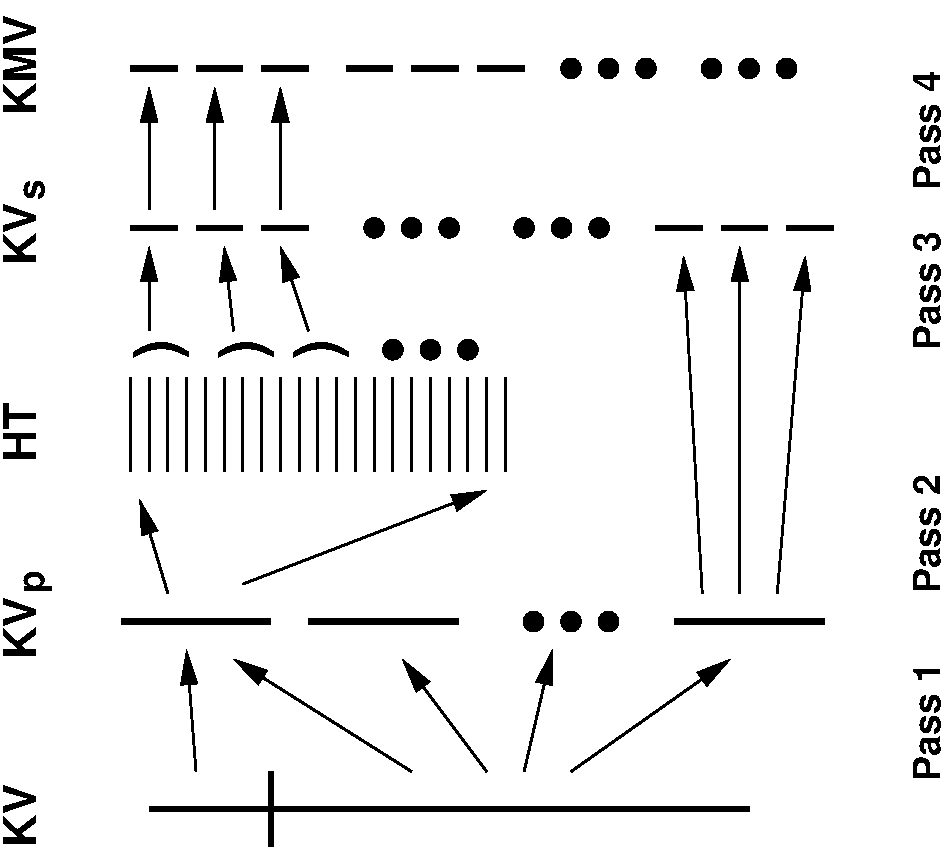
\includegraphics[width=\textwidth,angle=-90]{fig_collate2.pdf}
\caption{\it Multi-pass algorithm for converting KV data to KMV data.
The vertical lines represent out-of-core data sets.  KV is key/value
pairs; HT is an in-memory hash table; KMV is key/multivalue pairs.}
\label{fig:collate}
\end{figure}

\begin{itemize}

\item (Pass 1) The KV pairs are read, one page at a time, and split
into ``partition'' files, represented by KVp in the figure.  Each
partition file contains KV pairs whose unique keys (likely) fit
in the hash table (HT).  Initially, all KV pairs are assigned to the
first partition file as the HT is populated.  When the HT becomes
full, e.g. at the point represented by the horizontal line shown on
the leftmost vertical line as a downward scan is performed, the
fraction of KV pairs read thus far is used to estimate the number of
additional partition files needed.  As subsequent KV pairs are read,
they are assigned to the original partition file if the KV pair's
key is already in the current HT.  If not, a subset of bits in
the hash value of the key is used to assign the KV pair to one of the
new partition files.  The number of needed partition files is
estimated conservatively, rounding up to the next power-of-two, so
that extra passes through the KV pairs are almost never needed, and so
that the bit masking can be done quickly.  This first pass entails
both a read and write of all the KV pairs.

\item (Pass 2) The partition files are read, one at a time.  The key
for each KV pair is hashed into the HT, accumulating data about the
number and size of values associated with each unique key.  Before the
next partition file is read, passes 3 and 4 are completed for the
current partition.  Eventually this pass entails a read of all KV
pairs.

\item (Pass 3) The unique keys in the HT for one partition are
scanned to determine the total size of KMV for keys in the HT.  
The associated values create KMV pairs that span
$M$ memory pages.  If $M > 1$, the associated partition file of KV
pairs is read again, and each KV pair is assigned to one of $M$
smaller ``set'' files, represented by KVs in the figure.  Each set
file contains the KV pairs that contribute to the KMV pairs that
populate one page of KMV output.  If a single KMV pair spans
multiple pages because it contains a very large number of values,
the corresponding KV pairs are still written to a single set
file.  Eventually, this pass reads all partition files, entailing both
a read and write of all KV pairs.

\item (Pass 4) A set file is read and the key/value data for each of
its KV pairs is copied into the appropriate location in the page of
KMV pairs, using information stored in the HT.  When complete, the KMV
page is written to disk.  This pass eventually reads all set files,
entailing a final read of all KV pairs.  It also writes all KMV pairs
to disk.  If each KV pair has a unique key, the volume of KMV output
is roughly the same as that of the KV input.

\end{itemize}

In summary, this data reorganization for the {\it collate()} operation
is somewhat complex, but requires only a small, constant number of
passes through the data.  The KV datums are read from disk at most
four times, and written to disk three times.  The first two write
passes reorganize KV pairs into partition and set files; the final
write pass creates the KMV data set.  Depending on the size and
characteristics of the KV datums (e.g., the number of unique keys),
some of these passes may not be needed.  By contrast, a full
out-of-core sort of the KV pairs, performed via a merge sort as
discussed below is still an $O(N\log_2{N})$ operation.  The number of
read/write passes through the KV data files depends on the amount of
KV data that can be held in memory, but can be a large number for big
data sets.

The memory page requirements for the out-of-core {\it collate()}
operation are as follows.  Two contiguous pages of memory are used for
the hash table.  Intermediate passes 2 and 3 can require numerous
partition or set files to be opened simultaneously and written to.  To
avoid small writes of individual KV datums, a buffer of at least 16K
bytes is allocated for each file.  The precise number of
simultaneously open files is difficult to bound, but typically one or
two additional pages of memory suffice for all needed buffers.  Thus
the total number of pages required for the data reorganization stage
of the {\it collate()} operation is less than the seven used by the
all-to-all communication stage.

Other MR-MPI library calls discussed in the previous section, such as
{\it clone()}, {\it collapse()}, and {\it gather()}, can also operate
in out-of-core mode, typically with one pass through the KV or KMV
data and the use of one or two memory pages.  Sorting KV pairs, by key
or value, is an exception.  An out-of-core merge sort is performed as
follows.  Two pages of KV datums are read from disk.  Each is sorted
in local memory using the C-library quicksort() function, as discussed
in the previous section.  The two pages are then scanned and merged
into a new file which is written to disk as its associated memory page
fills up.  This process requires five memory pages, which includes
vectors of KV datum pointers and lengths needed by the in-memory
quicksort() operation.  Once all pairs of pages have been merged, the
sort continues in a recursive fashion, merging pairs of files into a
new third file, without the need to perform additional in-memory
sorts.  Thus the overall memory requirement is five pages.  The number
of read/write passes through the KV data set for the merge sort is
$O(\log_2{M})$, where $M$ is the number of pages of KV pairs.  The
number of passes could be reduced at the cost of allocating more
in-memory pages.
